% This is samplepaper.tex, a sample chapter demonstrating the
% LLNCS macro package for Springer Computer Science proceedings;
% Version 2.20 of 2017/10/04
%
\documentclass[runningheads]{llncs}
%
\usepackage{graphicx}
\usepackage{amsmath}
\usepackage{longtable}
\usepackage{float} % For precise float placement
\usepackage{subcaption} % For subtables
\usepackage{afterpage} % For forcing table to appear after current page
\usepackage{setspace} % For adjusting line spacing
\usepackage{dialogue}
\usepackage{xcolor}
% Used for displaying a sample figure. If possible, figure files should
% be included in EPS format.
%
% If you use the hyperref package, please uncomment the following line
% to display URLs in blue roman font according to Springer's eBook style:
% \renewcommand\UrlFont{\color{blue}\rmfamily}
% Used for a dialog representation

   
\begin{document}
%
\title{Conversational Task Agent}
%
%\titlerunning{Abbreviated paper title}
% If the paper title is too long for the running head, you can set
% an abbreviated paper title here
%
\author{Guilherme Fernandes\inst{1}\orcidID{60045} \and
Ricardo Silva\inst{1}\orcidID{60559} \and
Vladyslav Mikytiv\inst{1}\orcidID{60735}}
%
\authorrunning{Guilherme, Ricardo, Vladyslav}
% First names are abbreviated in the running head.
% If there are more than two authors, 'et al.' is used.
%
\institute{NOVA School Of Science and Technology}
%
\maketitle              % typeset the header of the contribution
%
\begin{abstract}
Our project focuses on creating an adaptive taskbot tailored specifically for guiding users through cooking tasks. This taskbot will utilize artificial intelligence and natural language processing to interact with users, understanding their progress and constraints in real-time. The taskbot will dynamically adjust instructions based on the ingredients and cooking tools available to the user. In instances where users encounter obstacles, such as running out of ingredients or lacking specific utensils, the taskbot will intelligently adapt the recipe, offering alternative ingredient substitutions or equipment alternatives to ensure successful completion of the dish. By providing personalised guidance our taskbot aims to enhance the culinary experience.

\keywords{Taskbot  \and Word embedding \and Natural Language Processing}
\end{abstract}
%
%
%
\section{Introduction}
In recent years, word embedding has emerged as a cornerstone technology in the field of artificial intelligence, revolutionising natural language processing (NLP) tasks. This transformative approach to representing words as dense vectors in continuous vector spaces has garnered significant attention and acclaim within the AI community. The rise of word embedding has been marked by its progression from conventional methods to the creation of sophisticated models capable of capturing intricate semantic connections among words.

The inception of word embedding can be traced back to the early 2000s when researchers began exploring methods to overcome the limitations of traditional vector space models, such as bag-of-words and one-hot encoding. These initial efforts paved the way for more advanced approaches that would later reshape the field of natural language processing (NLP).

However, it wasn't until the introduction of groundbreaking techniques like Word2Vec by Mikolov et al. in 2013 and GloVe (Global Vectors for Word Representation) by Pennington et al. in 2014 that word embedding started to gain widespread attention and adoption. These models introduced novel methodologies for learning distributed representations of words based on large corpora of text, capturing intricate semantic nuances and relationships.

The allure of word embedding lies in its ability to encode semantic meaning into dense vector representations, enabling machines to understand language in a more nuanced and contextually rich manner.

The project aims to utilize embedding algorithms and large language models to develop a dialog manager between users and the taskbot. This manager will execute user requests and guide them through processes, particularly in cooking recipes, with adaptability. Leveraging a dataset containing recipes data, including ingredients, procedural steps, and difficulty levels, we utilize OpenSearch indexing to efficiently retrieve information for user queries.


\section{Algorithms and Implementation}
\subsection{Indexing}
We must implement a search index of complex manual tasks in order to allow our system to retrieve relevant information about the tasks.

\begin{figure}[!htbp]
    \center
    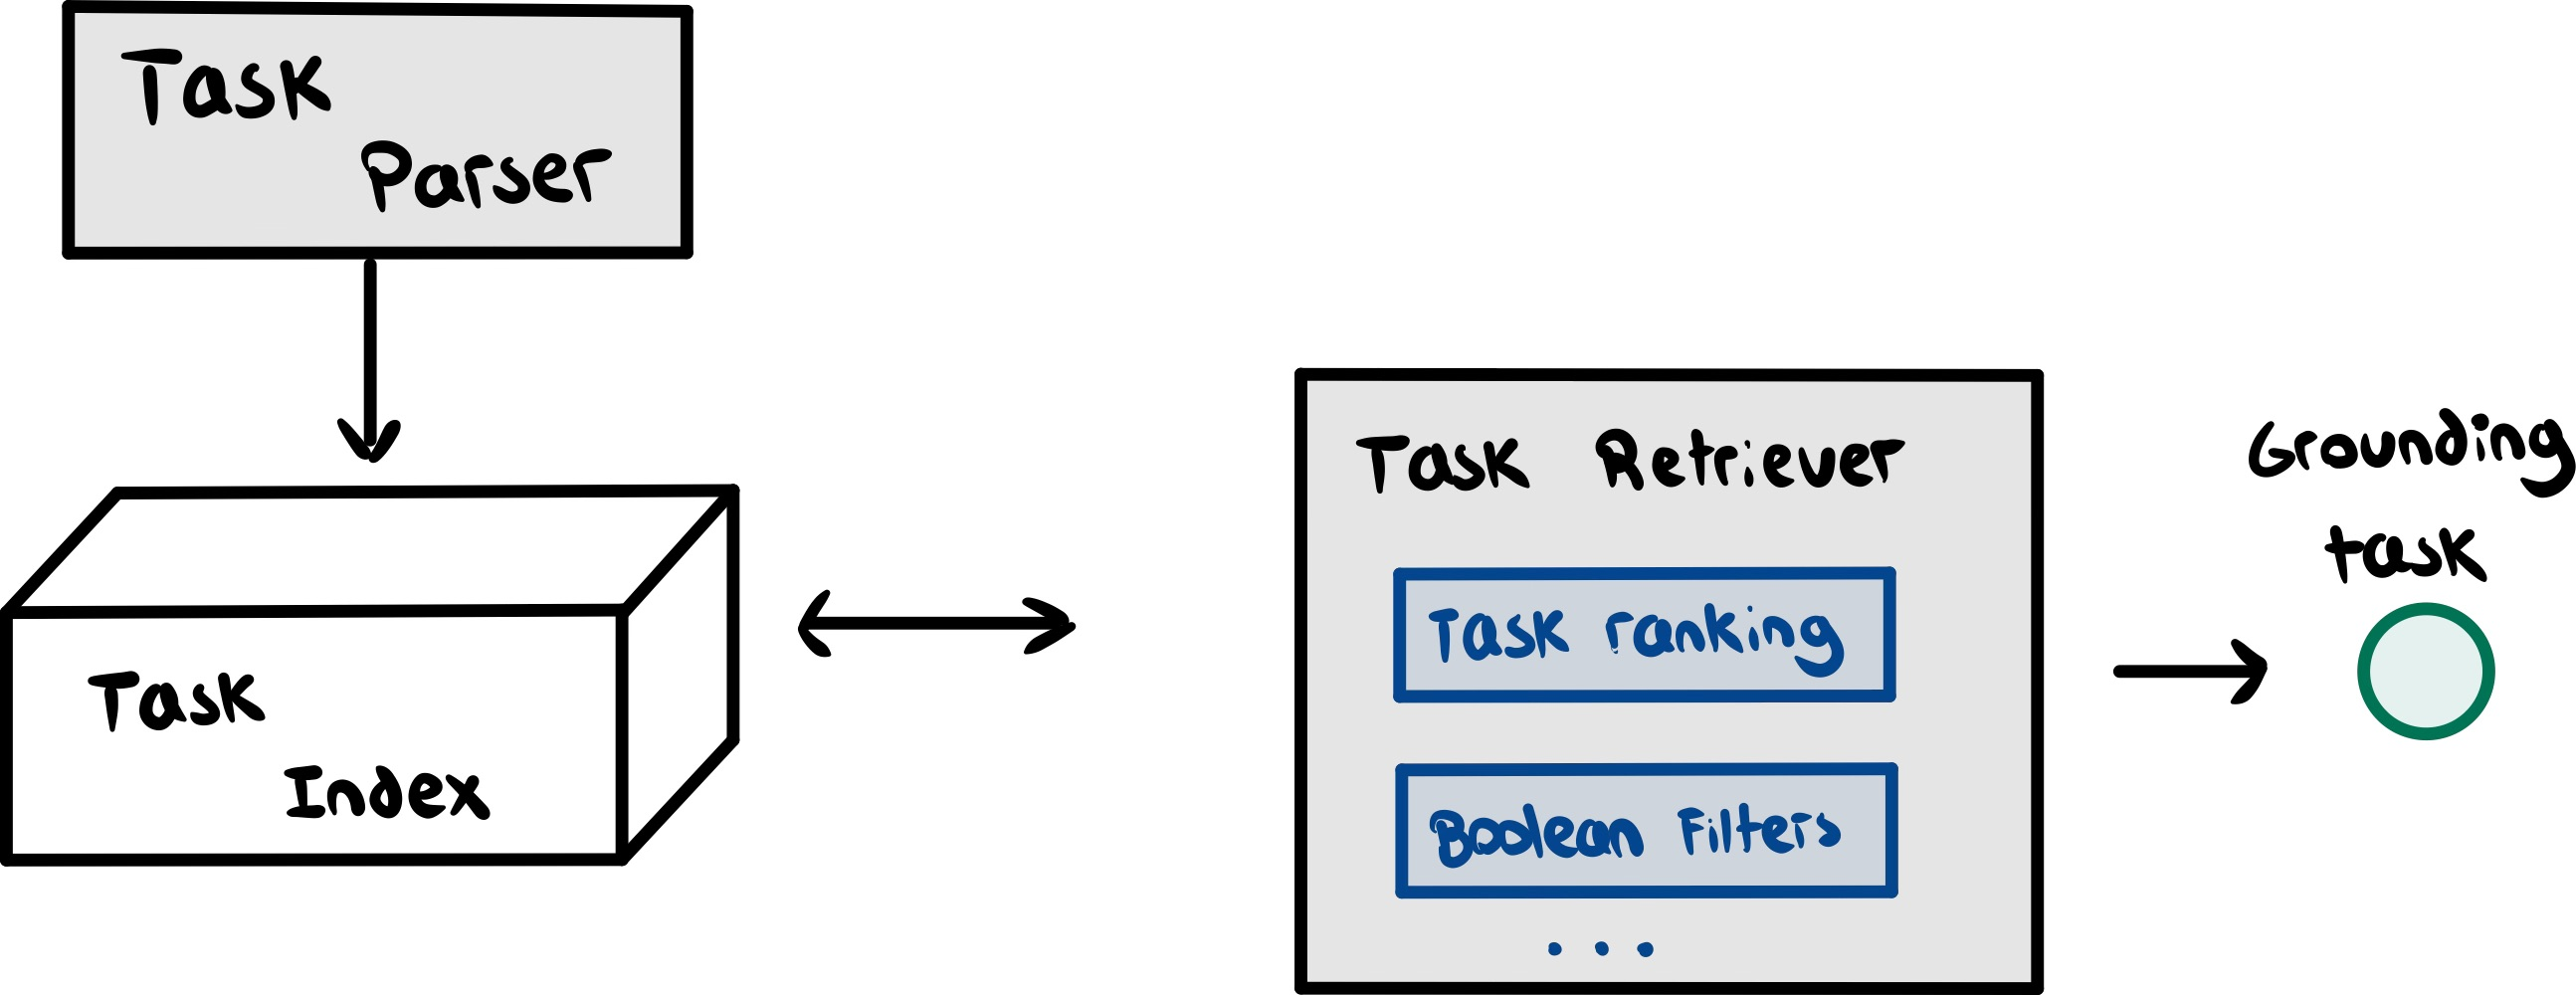
\includegraphics[scale=0.08]{images/task_retriever.jpg}
    \caption{Task retrieval}
\end{figure}

We must parse the data from the dataset which is a JSON file. We do that while we populate our indexes in OpenSearch. For each recipe we parse the JSON and send the relevant information to the index mapping that was created. We introduce a set of mappings tailored to effectively index recipe data and they are the following:

    
\begin{table}[ht]
\centering
\setlength{\abovecaptionskip}{10pt} % Adjust the spacing here
\resizebox{0.7\textwidth}{!}{%
\begin{subtable}{0.45\linewidth}
\centering
\begin{tabular}{|c|c|}
\hline
\textbf{Field} & \textbf{Data Type} \\ \hline
recipeJson & object \\ \hline
recipeName & text \\ \hline
prepTimeMinutes & integer \\ \hline
cookTimeMinutes & integer \\ \hline
totalTimeMinutes & integer \\ \hline
difficultyLevel & keyword \\ \hline
images & array of text \\ \hline
servings & float \\ \hline
\end{tabular}
\end{subtable}
\hfill % Add horizontal space between subtables
\begin{subtable}{0.45\linewidth}
\centering
\begin{tabular}{|c|c|}
\hline
\textbf{Field} & \textbf{Data Type} \\ \hline
videos & array of object \\ \hline
tools & array of text \\ \hline
cuisines & array of text \\ \hline
courses & array of text \\ \hline
diets & array of text \\ \hline
ingredients & array of object \\ \hline
stepsEmbedding & knn\_vector \\ \hline
\end{tabular}
\end{subtable}
}
\caption{Index Mapping}
\label{tab:mappings}
\end{table}

An important detail to emphasise is that our \textbf{ingredients} are a \textbf{nested type} with the properties \textbf{name} and most importantly the
corresponding \textbf{\text{ingredient\_embedding}}. We also used the mpnet-base-v2 transformer because it had better results.~\cite{mpnet}.

\subsection{Searching}
We've initiated the project by focusing on leveraging indexes for efficient dataset navigation, and OpenSearch emerges as a pivotal tool for executing queries seamlessly.

We've commenced with text-based queries, enabling users to access recipes based on various parameters such as cooking time, difficulty level, course type, or serving size.

Moreover, the integration of boolean queries adds another layer of flexibility, empowering users to refine their searches by specifying ingredients they desire or wish to avoid in their recipes.

Embedded queries stand out as particularly intriguing among our query types. By transforming user inputs into vector representations, we can uncover recipes closely related to the query. This method offers personalised recipe recommendations that align with users' interests more effectively.

In our index mappings, we utilize various embeddings to facilitate our searches. A crucial component is a model, referenced as~\cite{bert}, which extracts relevant information from natural language phrases, particularly focusing on ingredient extraction from user queries. This model also aids in processing the textual content within recipe steps.

Acknowledging the significance of recipe steps, we've introduced embeddings for both the recipe names and their corresponding individual steps. This approach enables our search system to capture the essence of each recipe efficiently, ensuring accurate query results.

After thorough testing, we've identified the most effective embeddings for our system: ingredient embeddings for individual ingredients and step embeddings paired with respective recipe names. Despite transformer limitations, these embeddings show promising results, especially in user-input based embedded queries. Given that our system doesn't prioritize contextual nuances in phrases, we've opted to utilize FoodBERT~\cite{bert} to maintain consistency with this approach.

In essence, our framework enables a dynamic exploration of the dataset, granting users the ability to refine their searches precisely according to their preferences and specific requirements.

\subsection{Vision Models}
Our system currently excels in recipe searches, but what about images? Incorporating image queries would greatly enhance its functionality. To achieve this, we require a vision model like CLIP~\cite{clip} that enables us to seamlessly integrate image searches into our system. CLIP is a vision model encoder that facilitates the computation of semantic similarity between a sentence and an image.

CLIP features a dual encoder architecture comprising of an \textbf{image encoder}, responsible for generating embedding vectors for images, and the \textbf{text encoder}, which produces embedding vectors for text. Notably, the text encoder's embeddings are contextualized within the realm of images, offering representations of text within an image context. This design enables comparisons between text and images, images and text, as well as images and other images.

To enable this functionality, we've revised our OpenSearch index mapping to accommodate these types of embeddings. Specifically, we've introduced a new embedding that combines the recipe name with its corresponding image. As a result, our index mapping table has been updated as follows:

\begin{table}[ht]
\centering
\setlength{\abovecaptionskip}{10pt} % Adjust the spacing here
\resizebox{0.7\textwidth}{!}{%
\begin{subtable}{0.45\linewidth}
\centering
\begin{tabular}{|c|c|}
\hline
\textbf{Field} & \textbf{Data Type} \\ \hline
recipeJson & object \\ \hline
recipeName & text \\ \hline
prepTimeMinutes & integer \\ \hline
cookTimeMinutes & integer \\ \hline
totalTimeMinutes & integer \\ \hline
difficultyLevel & keyword \\ \hline
images & array of text \\ \hline
servings & float \\ \hline
\end{tabular}
\end{subtable}
\hfill % Add horizontal space between subtables
\begin{subtable}{0.45\linewidth}
\centering
\begin{tabular}{|c|c|}
\hline
\textbf{Field} & \textbf{Data Type} \\ \hline
videos & array of object \\ \hline
tools & array of text \\ \hline
cuisines & array of text \\ \hline
courses & array of text \\ \hline
diets & array of text \\ \hline
ingredients & array of object \\ \hline
stepsEmbedding & knn\_vector \\ \hline
\bfseries\colorbox{yellow}{imageEmbedding} & knn\_vector \\ \hline
\end{tabular}
\end{subtable}
}
\caption{Updated Index Mapping}
\label{tab:mappings}
\end{table}

These embeddings incorporate the recipe title, not just the raw image, we observed improved query responses with this approach. To implement this, we've developed a KNN search mechanism that accepts either an image or text input. Initially, it performs a KNN search on the title embedding, retrieving the top results. Subsequently, we mix these results with another KNN search, which operates on the image embedding. This allows us to get the best results from both KNN searches. Since CLIP performs better with natural language, we enhance the embedding of recipe titles by prefixing the text with \textbf{"A photo of"}. This addition creates a more natural and descriptive phrase, aligning with the contextual understanding of CLIP's model.

With these new embeddings, users can now input either an image or text. For image inputs, we search in the embedding space to find recipes with the highest similarity scores. Similarly, text inputs are encoded using CLIP to compare with image embeddings, enabling retrieval of recipes whose images closely match the user's initial text query. 


Given that we store this data in OpenSearch, performing a KNN search also returns the images associated with the recipes. This architecture allows us to retrieve images not only from image queries but also from text queries. As a result, we can seamlessly access images corresponding to the search query, whether it's a text input or an image input.

It's worth highlighting that the original embeddings are distinct from the newly generated ones via CLIP. These CLIP text embeddings are specifically tailored for integration within an image-oriented context. 

We've significantly expanded our capabilities for returning recipes, starting from basic queries and progressing to more complex ones. Initially, we utilize simple queries and a straightforward embedding method for KNN searches. With the recent integration of CLIP, our capabilities have expanded further. Now, we can conduct image queries and text queries within the context of images, leveraging CLIP's advanced features for enhanced accuracy and relevance.

\subsection{Large Language Model: PlanLLM}
After retrieving a recipe, we will want to work with the specific recipe the user selected. For that we will use the aid of a large language model. PlanLLM is a conversational assistant trained to assist users in completing a recipe from beginning to end and be able to answer any related or relevant requests that the user might have ~\cite{planllmeacl24}

To integrate PlanLLM into our project, we need to manage a JSON file, which is then sent to a PlanLLM API. This API returns the PlanLLM's response based on the user's query. The manipulation and updating of the JSON file are managed by our system. When a user selects a recipe, we narrow our focus to the context of that specific recipe, guiding the user through the steps needed to reach the end goal.

The user can talk with the PlanLLM and receive answers such as:\\[5pt]

\hspace{0.5cm} % Adjust the value as needed for the desired horizontal shift
\begin{minipage}{1.2\textwidth} % Adjust width as needed
\begin{dialogue}
\speak{User} Let's begin the task! 
\speak{PlanLLM} Hi! How can I assist you today? 
\speak{User} What do I need to do?
\speak{PlanLLM} You are in the first step, preheat the oven to 350 degress.
\speak{User} Done! Let's move to the next step.
\speak{PlanLLM} Step 2: Mix the ingredients together.
\speak{User} In which step are we?
\speak{PlanLLM} We currently on Step 2: Mix the ingredients together.\\[5pt]
\end{dialogue}
\end{minipage}

We want to allow the user to take a photo of what he's currently doing, such as cutting tomatoes for a recipe, and we want the PlannLLM to figure out which step we're at and what we're doing. And since the PlanLLM isn't trained to directly process images we implemented an intermediate processing step to handle such cases. This involves transforming user-input images into text representations using CLIP. By comparing the embeddings of the image with the textual descriptions of each recipe step, we can determine which step the image corresponds to. This intermediary step ensures that images can be effectively incorporated into the recipe guidance process.

\begin{figure}[!htbp]
    \center
    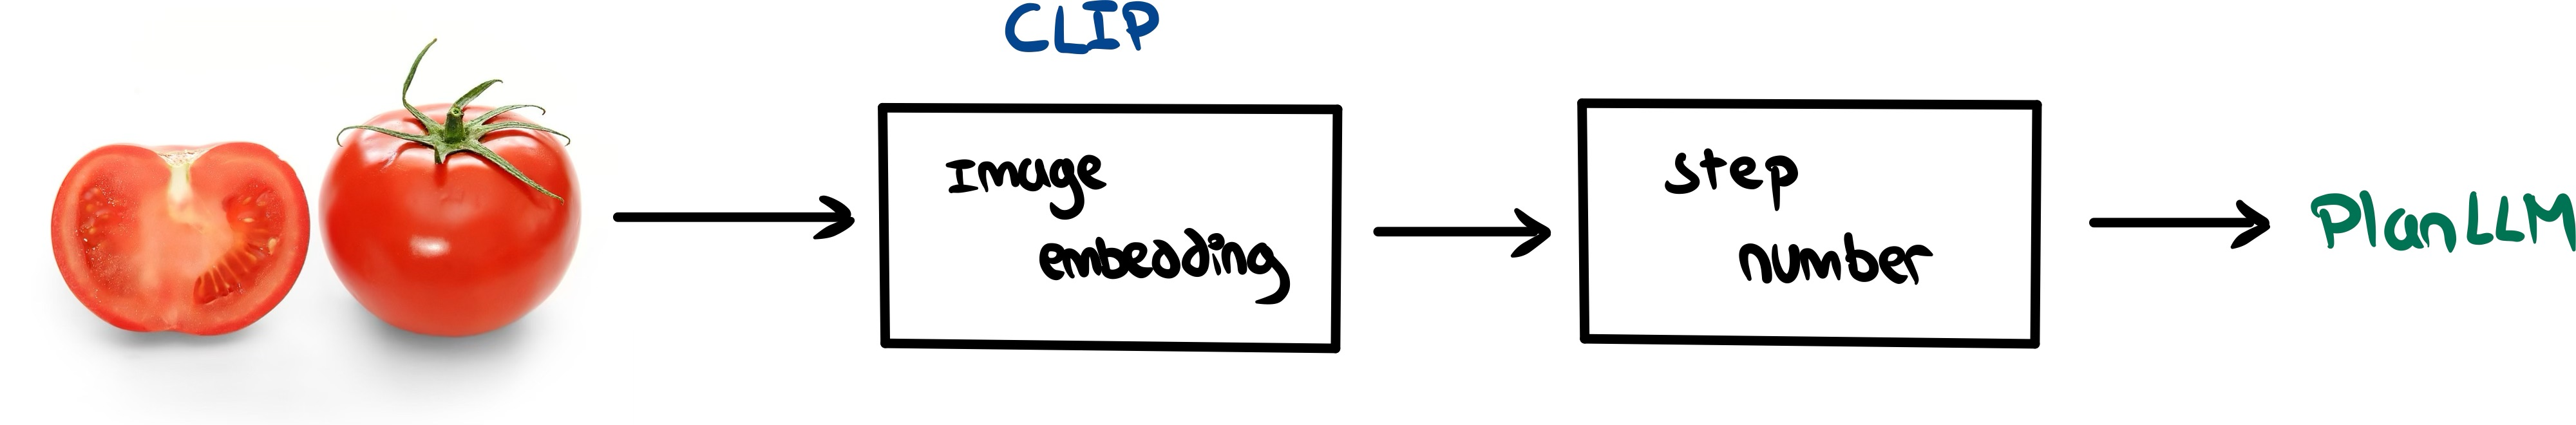
\includegraphics[scale=0.08]{images/planLLM.jpg}
    \caption{Image passing to PlanLLM}
\end{figure}

In order to re-create a conversation like the one above we need to carefully manipulate the JSON to get the answers we want. We've observed that PlanLLM struggles with transitioning between non-consecutive steps, such as starting from step 5 instead of step 1. However, the model responds effectively when the user provides a precise instruction like \textbf{"I am currently on step x"}. In such cases, we update the internal state to reflect the specified step provided by the user.

To achieve a more fluid and natural conversation flow, we've implemented a mechanism that enables users to provide either text or images as input. Using CLIP, we predict the step in the recipe that the user is referring to by comparing embedding scores and identifying the most relevant match. This approach allows users to jump between steps as desired through a simple photo of what they're currently doing, without the constraint of needing to use specific phrases like \textbf{"I am currently on step x"}. With this functionality in place, the remaining task is to orchestrate the entire dialogue with the user, which we'll cover in the next chapter.

\subsection{Contextual Embedding and Self-Attention Analysis}
\subsubsection{Contextual Embeddings:}
Let's analyse the contextual embedding of two phrases and look at the evolution in layers.

\begin{figure}[!htbp]
    \center
    \includegraphics[scale=0.2]{images/contextual\_embeddings}
    \caption{Contextual embeddings over layers}
\end{figure}
As we observe the evolution of the model's layers, we notice that tokens closely related to each other tend to cluster together, distinct from other tokens. With deeper layers, the model becomes adept at capturing intricate and abstract semantic relationships among words and phrases. This capability enables it to form more precise clusters based on nuanced semantic meanings, rather than just surface-level similarities. Furthermore, as we advance through the layers, the model gains access to more contextual information, further enhancing its ability to understand and process language.\subsubsection{Positional Embeddings:}
In here let's analyse a simple BERT encoder and we will work with a sequence text with the same word repeated 20 times.\\[10pt]

\begin{figure}[!htbp]
    \center
    \includegraphics[scale=0.3]{images/positional\_embeddings}
    \caption{Positional embeddings of a text with the same word}
\end{figure}

Here, we notice that the diagonal elements have a similarity score of 1, which is unsurprising as they represent comparisons of each position with itself. As we traverse away from the diagonal, the similarity score decreases, indicating that the words are farther apart in position. Notably, in the middle of the matrix, we observe a distinct division between the right and left sides. However, a deeper analysis of the first row and column is necessary to fully understand their behaviour.\subsubsection{Self Attention:} 
Here we will explore the differences between the \textbf{cross encoder} and \textbf{dual encoder} architectures.

In cross encoders we not only compute the self-attention, but we also compute the co-attention.
That is, we compute the attention between our input Query and the Key values, in order to force our model to relate both text sequences directly. This allows our model to grasp more detailed relations rather than just comparing the embeddings of each independently encoded sentence (also computed in the Query-Query relation, and Key-Key).
This is helpful because it allows our model to capture more intricate connections between the input texts. It can identify how the meaning of a token is influences by the presence of another token in the other text.

\begin{figure}[htbp]
    \centering
    \begin{minipage}{0.50\textwidth}
        \centering
        \includegraphics[width=\linewidth]{images/self\_attention\_matrix.png}
        \caption{Self Attention Matrix}
        \label{selfAttention}
    \end{minipage}\hfill
    \begin{minipage}{0.4\textwidth}
        \centering
        \includegraphics[width=\linewidth]{images/self\_attention\_class.jpg}
        \caption{Self Attention Matrix Showed in Class}
         \label{selfAttentionClass}
    \end{minipage}
\end{figure}

As we can see in Figure \ref{selfAttention} we can clearly see the separations on the matrix into four squares and each one of them indicates a self attention matrix. The matrix resembles the self attention matrix talked in class.

We can see that Figure \ref{selfAttentionClass} resembles the matrix present in Figure \ref{selfAttention}.

 As for the dual encoder both the sentences are encoded independently therefore resulting into different results. The advantage of this compared to the cross encoding is that the computational requirements aren't as big compared to the cross encoders. 

\begin{figure}[htbp]
    \centering
    \begin{minipage}{0.50\textwidth}
        \centering
        \includegraphics[width=\linewidth]{images/dual\_encoder2.png}
        \caption{Self Attention for Key}
         \label{dual1}
    \end{minipage}\hfill
    \begin{minipage}{0.50\textwidth}
        \centering
        \includegraphics[width=\linewidth]{images/dual\_encoder1.png}
        \caption{Self Attention for Query}
         \label{dual2}
    \end{minipage}
\end{figure}

In the embeddings of Figures \ref{dual1} and \ref{dual2} the embedding are calculated independently.
By passing the same two phrases to both these types of encodings we will get different results based on the architecture chosen, let's explore why is that.\\[5pt]

\hspace{0.5cm} % Adjust the value as needed for the desired horizontal shift
\begin{minipage}{1.2\textwidth} % Adjust width as needed
\begin{dialogue}
\speak{Text1} "How to make pasta?"
\speak{Text2} "How much 1KG of pasta costs?"\\[5pt]
\end{dialogue}
\end{minipage}

When we perform dual encoding, we encode each phrase separately and then calculate the similarity score between them. Using the encoder described in~\cite{reimers-2019-sentence-bert}, we might obtain an approximate score of 0.72 for two phrases discussing pasta but in different contexts. However, with cross encoding using the same model, both phrases are encoded within the same context. Consequently, the embeddings take into account the context of both phrases, resulting in a lower similarity score. This outcome is reasonable as the phrases, although mentioning pasta, are discussing different topics.
\section{Evaluation}
\subsection{Dataset Description}
The dataset contains a significant amount of recipe information, but not all of it is pertinent to our objectives. After careful examination, we have identified the essential data required for generating meaningful embeddings and providing accurate search results to users. Our focus has been on excluding irrelevant information and prioritizing specific details that enhance the user's search experience.

Following a thorough dataset analysis, we selectively filtered the essential data required for crafting our embeddings and information pertinent to users for search results. Our assessment highlighted the necessity for detailed information on certain aspects while deeming others less crucial.

During our process of embedding sentences and experimenting with various techniques, we encountered two significant problems. Firstly, the \textbf{displayText} of each ingredient contained excessive information, including opinions and irrelevant text. Secondly, some \textbf{displayText} entries were in languages other than English (e.g., Italian). This posed challenges, as searching for ingredients like Italian cheese would erroneously suggest a strong relationship due to language inconsistencies.

Therefore, to address these issues, we implemented two solutions. Firstly, we opted to utilize only the \textbf{ingredient} property of each ingredient. To accomplish this, we employed a model that extracts the ingredient from the \textbf{displayText} and populates the ingredient field in the JSON.

For that, we used the \url{https://github.com/strangetom/ingredient-parser}~\cite{ingredientParser} in order to extract the ingredients from a phrase. With this we solved the issue of having \textbf{null} values in these fields. However, the problem persisted with \textbf{textDisplay} being in another language, as the ingredient parser model~\cite{ingredientParser} simply returned the \textbf{displayText} as it was originally.

By utilizing a translator model~\cite{deeptranslate} before feeding the data to the ingredient parser~\cite{ingredientParser}, we successfully translated the \textbf{displayTexts} that were in other languages into English. This allowed us to apply the model to extract the ingredients and populate the missing fields.

These modifications to our original dataset resulted in a more comprehensive dataset. We created a new JSON file containing all of the original information along with the additional data. This file is accessible through OpenSearch, as it is stored without being indexed. Its sole purpose is to be retrievable from OpenSearch.

\subsection{PlanLLM Description}
Every step in our recipes have their respective embeddings encoded with CLIP, we generate these offline and store them locally for later consultation. Additionally, some steps have images associated with them, and we also store the embeddings of these images locally. When we're working within the context of a recipe, we retrieve the necessary similarities by computing the similarity score with CLIP using the inner product. We made the decision to handle this locally to avoid imposing unnecessary overhead on OpenSearch, as it seemed more efficient to manage this task outside of the OpenSearch environment.

As we engage in dialogue with PlanLLM, each API response triggers an update to our JSON file, which acts as our conduit for communication with PlanLLM. This ongoing updating ensures that our JSON file always reflects the latest context and information, ready to be utilised in subsequent conversations with PlanLLM. This dynamic process enables us to maintain coherence and continuity in our interactions with PlanLLM throughout the conversation.
\bibliographystyle{plain}
\bibliography{my_bib}

\end{document}
